%
% This is a borrowed LaTeX template file for lecture notes for CS267,
% Applications of Parallel Computing, UCBerkeley EECS Department.
% Now being used for CMU's 10725 Fall 2012 Optimization course
% taught by Geoff Gordon and Ryan Tibshirani.  When preparing 
% LaTeX notes for this class, please use this template.
%
% To familiarize yourself with this template, the body contains
% some examples of its use.  Look them over.  Then you can
% run LaTeX on this file.  After you have LaTeXed this file then
% you can look over the result either by printing it out with
% dvips or using xdvi. "pdflatex template.tex" should also work.
%

\documentclass[twoside]{article}
\setlength{\oddsidemargin}{0.25 in}
\setlength{\evensidemargin}{-0.25 in}
\setlength{\topmargin}{-0.6 in}
\setlength{\textwidth}{6.5 in}
\setlength{\textheight}{8.5 in}
\setlength{\headsep}{0.75 in}
\setlength{\parindent}{0 in}
\setlength{\parskip}{0.1 in}

%
% ADD PACKAGES here:
%

\usepackage{amsmath,amsfonts,graphicx}
\usepackage{tikz}

%
% The following commands set up the lecnum (lecture number)
% counter and make various numbering schemes work relative
% to the lecture number.
%
\newcounter{lecnum}
\renewcommand{\thepage}{\thelecnum-\arabic{page}}
\renewcommand{\thesection}{\thelecnum.\arabic{section}}
\renewcommand{\theequation}{\thelecnum.\arabic{equation}}
\renewcommand{\thefigure}{\thelecnum.\arabic{figure}}
\renewcommand{\thetable}{\thelecnum.\arabic{table}}

%
% The following macro is used to generate the header.
%
\newcommand{\lecture}[4]{
   \pagestyle{myheadings}
   \thispagestyle{plain}
   \newpage
   \setcounter{lecnum}{#1}
   \setcounter{page}{1}
   \noindent
   \begin{center}
   \framebox{
      \vbox{\vspace{2mm}
    \hbox to 6.28in { {\bf CPSC 313: Introduction to Computability
	\hfill Fall 2016} }
       \vspace{4mm}
       \hbox to 6.28in { {\Large \hfill Lecture #1: #2  \hfill} }
       \vspace{2mm}
       \hbox to 6.28in { {\it Lecturer: #3 \hfill Scribe: #4} }
      \vspace{2mm}}
   }
   \end{center}
   \markboth{Lecture #1: #2}{Lecture #1: #2}


}
%
% Convention for citations is authors' initials followed by the year.
% For example, to cite a paper by Leighton and Maggs you would type
% \cite{LM89}, and to cite a paper by Strassen you would type \cite{S69}.
% (To avoid bibliography problems, for now we redefine the \cite command.)
% Also commands that create a suitable format for the reference list.
\renewcommand{\cite}[1]{[#1]}
\def\beginrefs{\begin{list}%
        {[\arabic{equation}]}{\usecounter{equation}
         \setlength{\leftmargin}{2.0truecm}\setlength{\labelsep}{0.4truecm}%
         \setlength{\labelwidth}{1.6truecm}}}
\def\endrefs{\end{list}}
\def\bibentry#1{\item[\hbox{[#1]}]}

%Use this command for a figure; it puts a figure in wherever you want it.
%usage: \fig{NUMBER}{SPACE-IN-INCHES}{CAPTION}
\newcommand{\fig}[3]{
			\vspace{#2}
			\begin{center}
			Figure \thelecnum.#1:~#3
			\end{center}
	}
% Use these for theorems, lemmas, proofs, etc.
\newtheorem{theorem}{Theorem}[lecnum]
\newtheorem{lemma}[theorem]{Lemma}
\newtheorem{proposition}[theorem]{Proposition}
\newtheorem{claim}[theorem]{Claim}
\newtheorem{corollary}[theorem]{Corollary}
\newtheorem{definition}[theorem]{Definition}
\newenvironment{proof}{{\bf Proof:}}{\hfill\rule{2mm}{2mm}}

% **** IF YOU WANT TO DEFINE ADDITIONAL MACROS FOR YOURSELF, PUT THEM HERE:

\newcommand\E{\mathbb{E}}

\begin{document}
%FILL IN THE RIGHT INFO.
%\lecture{**LECTURE-NUMBER**}{**DATE**}{**LECTURER**}{**SCRIBE**}
\lecture{19}{Midterm Review}{Dr. Catalin Dohotaru}{Shane Sims}
%\footnotetext{These notes are partially based on those of Nigel Mansell.}

% **** YOUR NOTES GO HERE:

% Some general latex examples and examples making use of the
% macros follow.  
%**** IN GENERAL, BE BRIEF. LONG SCRIBE NOTES, NO MATTER HOW WELL WRITTEN,
%**** ARE NEVER READ BY ANYBODY.

Add some intro for the notes here about the general method of reduction and how this fits into what we learned in the last  two lectures

\section{Reduction: A first example} % Don't be this informal in your notes!

\begin{theorem}
The language Halt =  \{$\langle M, w \rangle |$ M halts on input w\} is undecidable.
\end{theorem}

\begin{proof}
Suppose for contradiction, that the language Halt, is not undecidable. Then there is a Turing Machine, denoted H, deciding Halt. 

Proof Idea: From this reductio assumption, it will be shown that we can can use H to build another TM, SH that decides the language SelfHalt (seen last lecture). But since we have proved SelfHalt to be undecidable, we will have discovered a contradiction. This contradiction negates our assumption and proves that in fact, Halt is also undecidable.

We use H to build a machine SH as follows: Given any string w, the machine SH should first verify that $w = \langle M \rangle$ for some Turing Machine M (and rejects otherwise). Then SH writes the string $ww = \langle M, M \rangle$ and passes it to H. Thus we have described a machine that decides SelfHalt, using our assumption that Halt is decidable. But this is impossible as shown in last lecture. So we have a contradiction and have proven that Halt is undecidable, as required.  

\end{proof}

\subsection{Reduction by Formal Definition}
\begin{figure}[h!]
\centering
\begin{tikzpicture}
\pgftext{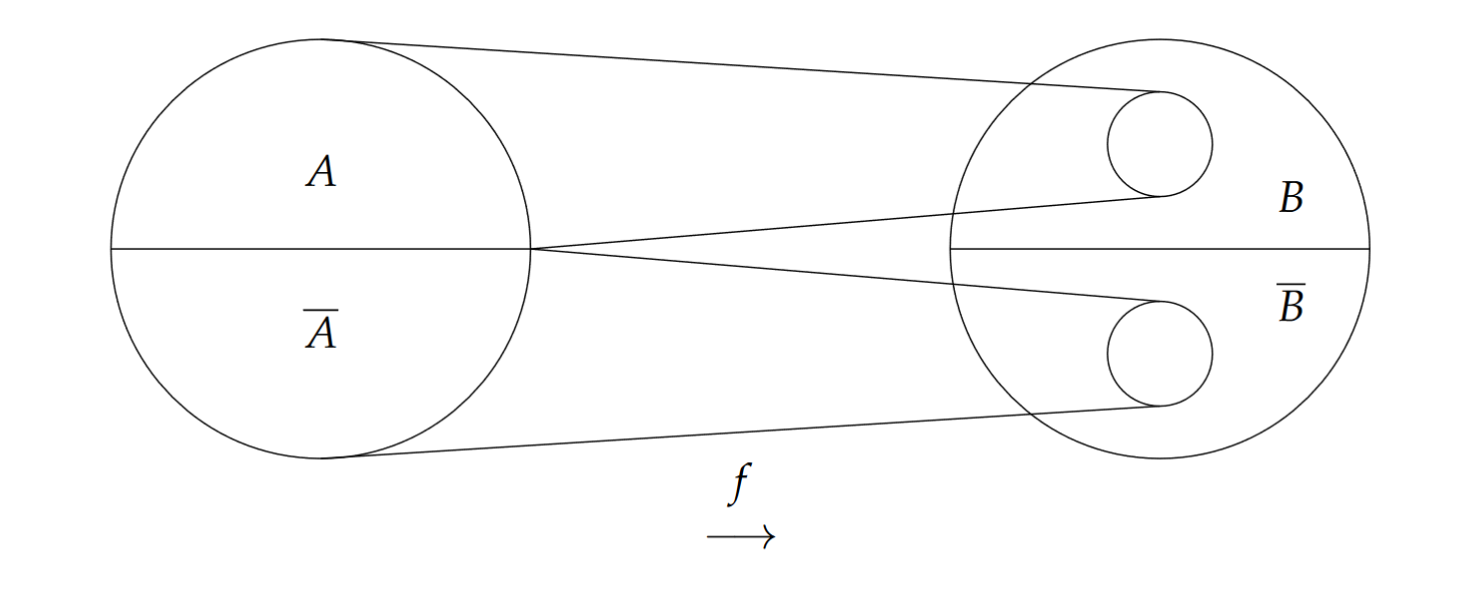
\includegraphics[width=350pt]{redAtoB.png}} at (100pt,100pt);
\end{tikzpicture}
\caption{A reduction, $f$, from A to B } \label{A reduction, $f$, from A to B }
\end{figure}
\begin{definition}


A function $f: \Sigma^* \rightarrow \Sigma^*$ is a \textbf{computable function} if there exists a Turing Machine that, for every input $w\in \Sigma^*$, halts with $f(w)$ written on its tape. 

Note: We say that language A \textbf{reduces} to language B, denoted $A \leq_m B$ if there exists a computable reduction from \textbf{A} to \textbf{B}.
\end{definition}

\begin{theorem}
If $A \leq_m B$ and A is undecidable, then so is B.
\end{theorem}
\begin{proof}
Assume that B is decidable and let  $f: \Sigma^* \rightarrow \Sigma^*$ such that $w \in A \leftrightarrow$ $f(w) \in B$ for every $w \in \Sigma^*$. Let $M_B$ be a Turing Macine that decides B and $M_f$  be a Turing Machine that computes $f$. Then the following machine decides the language A:\newline
Operation of M on winput $w$:
\begin{enumerate}
\item Simulate  $M_f$ on $w$ to compute $f(w)$.
\item Simulate $M_B$ on $f(w)$.
\item Accept if $M_B$ accepts and reject if $M_B$ rejects.
\end{enumerate}
This contradicts the fact that A is not decidable.\newline
In general, to prove a that a language L is undecidable, reduce a known undecidable language to L. 
\end{proof}

\begin{theorem}
The language ANY = \{$\langle M \rangle | L(M)$ contains at least one string\} is undecidable.
\end{theorem}
Proof Idea: We know that HALT is undecidable (shown in 30.1). So if we can reduce HALT to ANY (i.e. $HALT \leq_m ANY$), then we will have shown taht ANY is undecidable by appealing to Theorem 30.3, without having to do any further work.\newline

\begin{proof}
Definition 30.2 tells us that HALT reduces to ANY if there exists a function $f$ such that $w \in HALT \leftrightarrow f(w) \in ANY$. That is: \newline
 If a string $w$ is an element of the language HALT, then its transformation under $f$ is an element of the language ANY. If $w \notin HALT$ then $f(w) \notin ANY$.\newline
 
 It remains to find $f$ as described in Definition 30.2:\newline
 First we define a Turing Machine, $M'$ as follows:\newline
 
 \hspace{1cm} On input $\langle M, w \rangle$, $M'$ will
 \begin{enumerate}
 \item Run M on input $w$.
 \item If M accepts $w$, then $M'$ accepts $w$.
 \item If M rejects $w$, then $M'$ \textbf{accepts} $w$.
 \item If M loops on $w$, then $M'$ loops on $w$.
 \end{enumerate}
 Now we define the function $f: \Sigma^* \rightarrow \Sigma^*$ as follows:\newline
 \begin{displaymath}
   f(x) = \left\{
     \begin{array}{lr}
       \langle M', w \rangle & : x = \langle M, w \rangle\\
       x &  otherwise
     \end{array}
   \right.
\end{displaymath}
 
 Now we can check to see if $f$ is a reduction from HALT to ANY.\newline
 Suppose we have input $\langle M, w \rangle \in HALT$. Then:\newline
 $\langle M, w \rangle \in HALT \rightarrow$ M halts on $w \rightarrow$ $M'$ accepts $w \rightarrow$ $M' \in ANY \rightarrow f(\langle M, w \rangle) \in ANY$.\newline
 
 Then we have that  $\langle M, w \rangle \in HALT$, then $f(\langle M, w \rangle) \in ANY$.\newline
 We must now show that If $f(\langle M, w \rangle) \in ANY$, then  $\langle M, w \rangle \in HALT$. But this is equivalent to $\langle M, w \rangle \notin HALT \rightarrow f(\langle M, w \rangle) \notin ANY$, which is more suitable to our purpose.\newline
 
Suppose we have $\langle M, w \rangle \notin HALT \rightarrow $ M does not halt on $w \rightarrow M'$ does not halt on $w \rightarrow M' \notin ANY \rightarrow  f(\langle M, w \rangle) \notin ANY$.\newline

Then $f$ is a reduction and $HALT \leq_m Any$, proving that ANY is undecidable, as required.
\end{proof}



% **** THIS ENDS THE EXAMPLES. DON'T DELETE THE FOLLOWING LINE:

\end{document}





